\documentclass[12pt]{article}
\usepackage[utf8]{inputenc}    % Character encoding
\usepackage{amsmath}           % Advanced math typesetting
\usepackage{geometry}          % Page layout
\usepackage{graphicx}          % Figures
\usepackage{fancyhdr}          % Custom headers/footers
\usepackage{sectsty}           % Section font customization
\usepackage{xcolor}            % Color support
\usepackage{listings}          % Code snippets
\usepackage{float}             % Floating environments
\usepackage{hyperref}          % Hyperlinks

% Geometry setup
\geometry{a4paper, margin=1in}

% Define colors
\definecolor{bgcolor}{RGB}{236, 236, 236}      % Background color
\definecolor{bodycolor}{RGB}{50, 50, 50}       % Body text color
\definecolor{titlecolor2}{RGB}{169, 32, 32}    % Section title color

% Set background and text colors
\pagecolor{bgcolor}
\color{bodycolor}

% Font settings
\renewcommand{\rmdefault}{cmr}     % Body font: Computer Modern serif
\renewcommand{\sfdefault}{cmss}    % Heading font: Computer Modern sans-serif
\allsectionsfont{\sffamily \color{titlecolor2}}  % Sans-serif headings in red

% Header/footer setup
\pagestyle{fancy}
\fancyhf{}
\rhead{CS/CE 412/471 $\mid$ Algorithms}    % Right header (customize as needed)
\lhead{Implementation Report}                 % Left header (customize as needed)
\cfoot{\thepage}                          % Page number in footer
\setlength{\headheight}{15.0pt}

% Listings setup for code
\lstset{
    basicstyle=\ttfamily\small,
    keywordstyle=\color{blue},
    commentstyle=\color{green!50!black},
    stringstyle=\color{red},
    breaklines=true,
    frame=single,
    numbers=left,
    numberstyle=\tiny\color{gray},
}

% Title and author setup
\author{Your Name(s)}                     % Customize author(s)
\date{\today}
\newcommand{\thetitle}{Dynamizing Dijkstra for Dynamic Shortest Paths}  % Customize title
\newcommand{\thedate}{\today}
\newcommand{\course}{CS/CE 412/471 Algorithms: Design \& Analysis}  % Customize course

\begin{document}

% Title page
\begin{titlepage}
    \centering
    \vspace*{3.5cm}
    % Uncomment and replace with your logo if needed
    % \includegraphics[scale=10]{Logosmall.png}\\[1.0cm]
    \textsc{\LARGE Habib University}\\[1.0cm]  % Customize institution
    \textsc{\large Rija Hasan, Zuhair Abbas, Adina Adnan}\\[0.5cm]      % Same as \author
    \rule{\linewidth}{0.2mm}\\[0.8cm]
    {
    \sffamily \huge \bfseries
    \linespread{1}\selectfont
    \begin{center}
        \parbox{0.9\textwidth}{\centering \thetitle}
    \end{center}
    \vspace*{0.4cm}
    }
    \rule{\linewidth}{0.2mm}\\[0.8cm]
    {\large \thedate}\\[1cm]
    \course\\                                  % Uses \course command
    Implementation Report
\end{titlepage}

% Main content
\section*{Implementation Summary}

We implemented the dynamic Dijkstra algorithm in Python based on the pseudocode provided in the paper. All of the algorithm is complete and tested, as we elaborate in the next section. It is worth mentioning that there were typos in the pseudocode (e.g: line 10 "Update estimated distance ($d[e_t]$) for the vertex $e_t$ in priority queue should have been to update $e_h$ aka the current distance we have travelled) which we went out of our way to correct. 

Let us begin with the main data structure for the algorithm: the retrospective priority queue (RPQ).

The RPQ is managed using red black trees, where nodes represent vertices and their associated information, such as distance, time of insertion, and predecessors.
It is divided into two trees: one for insertions ($T_ins$) and one for deletions ($T_{d\_m}$). The algorithm checks for conflicts between these two trees when edges are updated. When an edge’s weight is updated, the algorithm isolates that specific edge update instead of recalculating the entire graph. This is done by updating only the affected edges and their ancestors.
The cascading effect ensures that if an edge is part of the shortest path, its change propagates to all relevant ancestors, adjusting the distances accordingly. 

After updating an edge, the algorithm propagates changes to the ancestors of the affected vertex, revisiting previously processed nodes and checking for better paths.
Cascading updates ensure that the changes are applied incrementally, only affecting the nodes that are influenced by the updated edge. When an edge deletion causes a change in the shortest path, the relevant entries are marked as invalid, and the algorithm checks whether any of the previously invalidated entries need to be revived. 

The heart of the algorithm's efficiency is through only updating the necessary parts of the graph. By focusing on specific edge updates rather than recalculating the entire graph, it minimizes computation.


\section*{Correctness Testing}
Multiple tests were run to test the retroactive updates of the algorithm. These were divided into:
\begin{enumerate}
    \item Update edge \textbf{not involved} in any other shortest path 
    \item Update edge \textbf{involved} in the shortest path of ancestors
    \item \textbf{Reupdating} nodes and going back and forth in time
\end{enumerate}
We will be using the graph in \ref{fig:graph} to demonstrate the correctness our our algorithm. The initial distances calculated from the static Dijkstra algorithm are described in Snippet \ref{fig:initialdists}. 


\begin{figure}[h!]
    \centering
    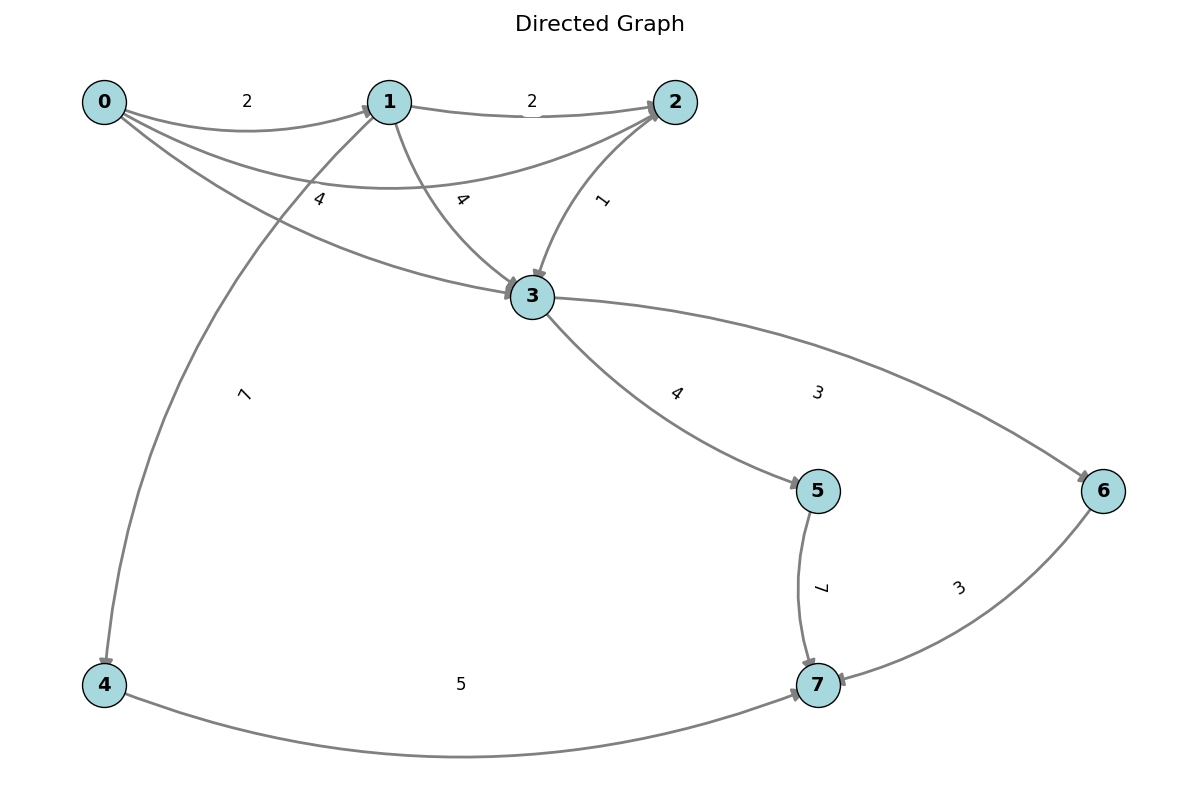
\includegraphics[width=0.6\textwidth]{graph.png}
    \caption{Graph for testing} 
    \label{fig:graph}
\end{figure}


\begin{figure}[h!]
    \centering
    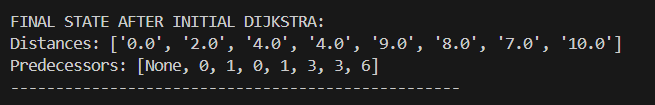
\includegraphics[width=0.6\textwidth]{initial distances.png}
    \caption{Initial Distances} 
    \label{fig:initialdists}
\end{figure}


\subsection*{Isolated Edges:}
We refer to edges that are not involved in any of the shortest paths as isolated edges. 
\begin{itemize}
    \item \textbf{Weight increases:} If the weight of such an edge increases, it should have no effect on any of the paths or predecessors recorded. This can be shown in Figure \ref{fig:isolated}. The increase of edge $(1,4)$ was not involved in the shortest path of other vertices. Hence, after the update, only the path to $4$ has changed.
    \item \textbf{Weight decreases:} If the weight of such an edge decreases, a new shortest path may be present to its ancestors. In this case, the effect is cascading as seen in figure \ref{fig:isolateddec}, the predecessor of 7 goes from 6 to 4. 
\end{itemize}
\begin{figure}[h!]
    \centering
    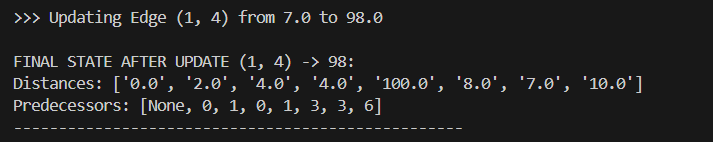
\includegraphics[width=0.6\textwidth]{isolated1.png}
    \caption{Isolated Edge (1,4) - Weight Increases} 
    \label{fig:isolated}
\end{figure}
\begin{figure}[h!]
    \centering
    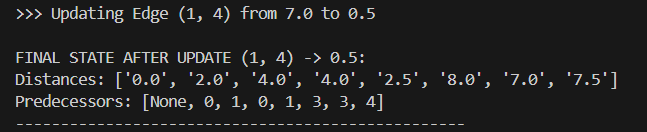
\includegraphics[width=0.6\textwidth]{isolateddec.png}
    \caption{Isolated Edge (1,4) - Weight Decreases} 
    \label{fig:isolateddec}
\end{figure}


\subsection*{Involved Edge:}
Involved edges are the ones that have been involved in the shortest path calculated before, and updating these may or may not have an effect on the shortest paths to other vertices. 
\begin{itemize}
    \item \textbf{Weight increases:} If the weight of an involved edge increases, it may have an effect on the shortest path predecessors of other vertices. This can be shown in Figure \ref{fig:cascading}. The increase of edge $(0,3)$ to 100 changes the paths to 5 and 6 and as a result, the predecessor of 7 becomes 4 from 6. This is the \textbf{cascading effect} where updates to one edge can lead to many other updates.
    \item \textbf{Weight decreases:} If the weight of an involved edge decreases, all predecessors remain the same, but the distances are updated in a cascading manner. This is shown in figure \ref{fig:cascadingdec} where the update of (0,3) to 1 now changes only the distances, not predecessors.
    
\end{itemize}


\subsection*{Repeated updates:}
Repeated updates entail going back in time to revoke deleted operations and propagate the changes to all vertices dependent on the update. This is shown in the figure in \ref{repeated} where edge (0,3) increases to 100, decreases to 1, and then increases to 100 again. In this case, the algorithm finds the deletion time of the vertex affected, 7 in this case, and rolls back the state to the previous distance and predecessor. This ensures that paths are not calculated repeatedly, but fetched from the right moment of time in the past. 

\begin{figure}[h!]
    \centering
    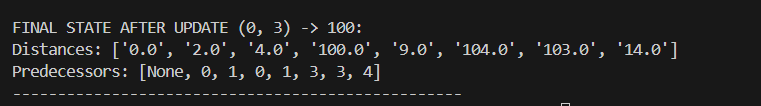
\includegraphics[width=0.6\textwidth]{cascading.png}
    \caption{Involved Edge (0,3) - Weight decreases} 
    \label{fig:cascading}
\end{figure}
\begin{figure}[h!]
    \centering
    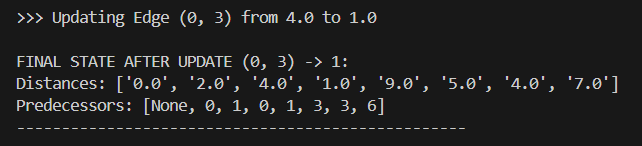
\includegraphics[width=0.6\textwidth]{cascadingdec.png}
    \caption{Involved Edge (0,3) - Weight decreases} 
    \label{fig:cascadingdec}
\end{figure}

\begin{figure}[h!]
    \centering
    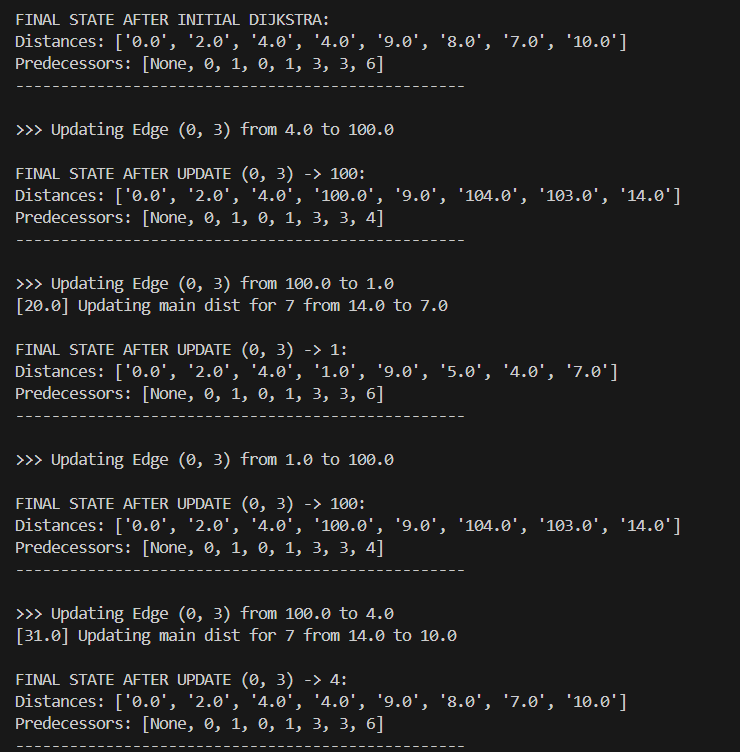
\includegraphics[width=0.6\textwidth]{repeated.png}
    \caption{Repeated Updates on node 3} 
    \label{repeated}
\end{figure}

\newpage

\subsection*{Visualization:}

Here is a visual example with the same graph as before. This was what was obtained after running an initial Dijkstra before updates.

\newpage

\begin{figure}[h!]
    \centering
    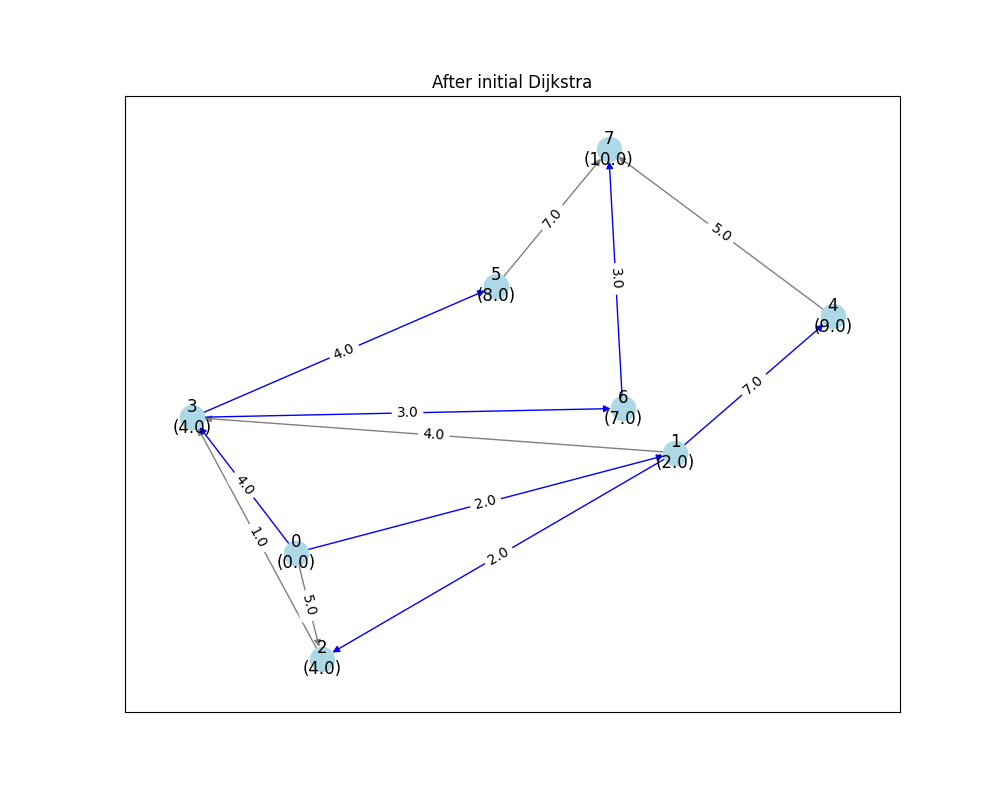
\includegraphics[width=0.75\textwidth]{After_initial_Dijkstra.png}
    \caption{Test graph's initial distances.} 
    \label{test_1}
\end{figure}

Let's say one of the distances gets updated. Specifically, edge (5, 7) morphs from a distance of 7.0 to 1.0 instead. The algorithm processes and updates accordingly to give a new shortest path to node 7.

\begin{figure}[h!]
    \centering
    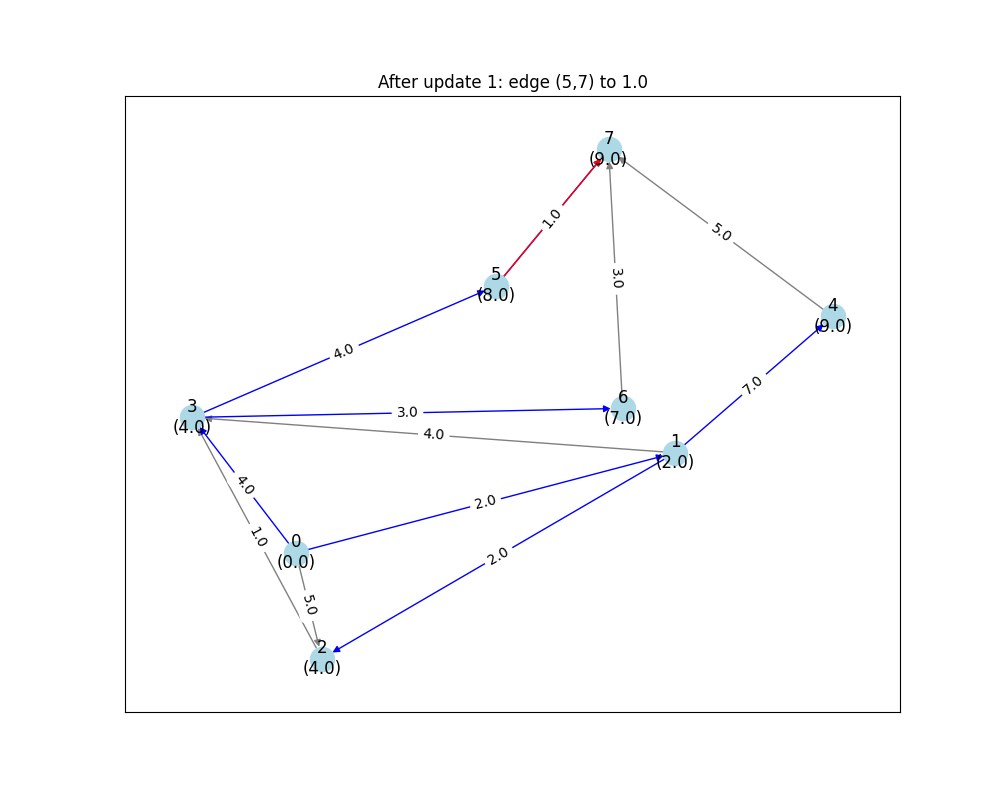
\includegraphics[width=0.75\textwidth]{After_update_1_edge_5,7_to_10.png}
    \caption{After updating (5, 7).} 
    \label{test_2}
\end{figure}

Similarly, we may update another edge (e.g: (3, 6)) from 3.0 to 1.5. This gives us a newer path to node 7.

\begin{figure}[h!]
    \centering
    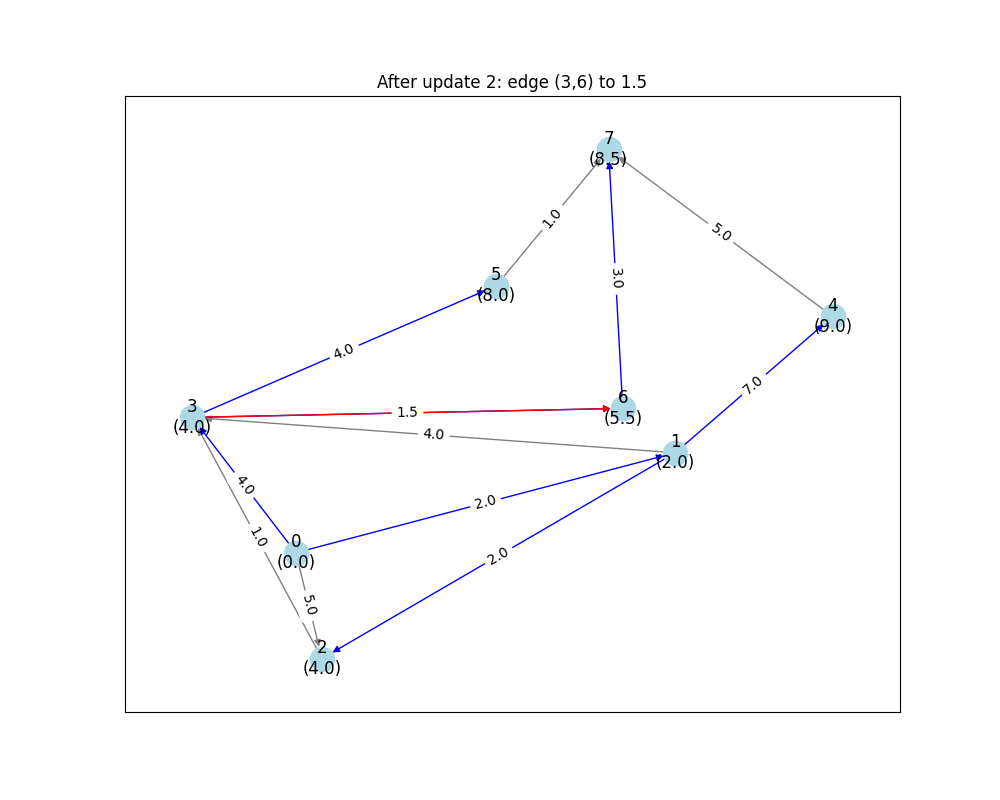
\includegraphics[width=0.75\textwidth]{After_update_2_edge_3,6_to_15.png}
    \caption{After updating (3, 6).} 
    \label{test_3}
\end{figure}

\section*{Complexity \& Runtime Analysis}

 First, let's look at the RPQ. The RPQ operations (insert, delete-min, decrease-key) take \(O(\log k)\), where \(k \leq V + E\), so roughly \(O(\log V)\).

In the worst case, an update (e.g., reducing a source-adjacent edge weight) impacts all \(V\) vertices, requiring \(V\) extract-mins and \(E\) decrease-keys. \(V\) extract-mins cost \(O(V \log V)\) and \(E\) decrease-keys cost \(O(E \log V)\). Summing these gives us:
\[
O(V \log V) + O(E \log V) = \mathbf{O((E+V) \log V)}
\]

What about the average case? Assume a sparse graph (\(E \approx V\)) and a balanced shortest path tree, where an update affects \(a = O(\log V)\) vertices (e.g., a subtree in a binary-like tree, averaged over depths). Operations include \(O(a)\) extract-mins and \(O(a)\) decrease-keys, each \(O(\log V)\), so we can freely consider both as the same. Our average-case complexity is \[O(a \log V) = O(\log V \cdot \log V) = \mathbf{O((\log V)^2)}\].

\section*{Baseline or Comparative Evaluation}

An obvious baseline is the standard or static Dijkstra algorithm. Traditionally, it takes $O(V^2)$; with a priority queue, it optimizes to $\mathbf{O((V+E)\log V)}$ for \textbf{any} update, not just the worst one.

From our prior analysis, While the worst-case complexity is the same as the optimized standard Dijkstra's algorithm, the dynamic Dijkstra shows its speedup in the average case of localized updates. So, in theory, dynamic Dijkstra is much more optimized for the average case than its static counterpart.


We have compared our algorithm with the baseline evaluation which is the approach that involves rerunning the Dijsktra algorithm after each update. The results are shown in the table below. The dynamic algorithm performs much better than the static version, especially when the graph becomes larger and the number of updates increase. The results are shown in the table below.

\begin{table}[h!]
\centering
\resizebox{\textwidth}{!}{%
\begin{tabular}{|c|c|c|c|c|}
\hline
\textbf{Vertices (n)} & \textbf{Edges (m)} & \textbf{Num of Updates} & \textbf{Time Taken by Static Dijkstra} & \textbf{Time Taken by Dynamic Dijkstra} \\
\hline
10 & 15 & 10 & 0.0000 & 0.0000 \\
20 & 30 & 20 & 0.0029 & 0.0000 \\
50 & 100 & 50 & 0.0010 & 0.0000 \\
100 & 200 & 150 & 0.0059 & 0.0010 \\
200 & 500 & 200 & 0.0207 & 0.00102 \\
\hline
\end{tabular}%
}
\caption{Comparison of Static and Dynamic Dijkstra's Algorithm}
\end{table}

\section*{Challenges \& Solutions}

We have faced significant challenges in the implementation of this algorithm, whether it be due to the complexity of the concept or the scalability of the solution.
\begin{itemize}
    \item \textbf{Paper's Description:} The pseudocodes present in the paper detail ambiguous functions that were extremely difficult to implement without any other sources on the material available. The figures in the charts had typos where entries changed, moving from one state to another without any logical progression. We dealt with this problem by discussing the approach amongst ourselves in coordinated sessions. 

    \item \textbf{Complexity:} Our initial algorithm did not actually utilize the RPQ as well as it should have. Though we did not perform a theoretical analysis of it, runtime results showed time taken similar to Dijkstra for larger graphs, which we found inadequate. This required a reevaluation of the algorithm to better fit the paper.

\item \textbf{Repeated Edge Updates:} Another challenge that was faced was managing repeated edge updates. When the weight of an edge is updated multiple times, it was causing inconsistencies in the graph’s state. The primary concern was to handle these repeated updates without recalculating the the shortest paths for the entire graph. To resolve this, we isolated the updates to only affected edges and vertices, using RPQ to track changes and propagate them efficiently. This approach prevented unnecessary recalculations and ensured consistency, allowing the system to handle multiple edge updates without restarting the entire process.

\end{itemize}



\section*{Enhancements}

\begin{itemize}
\item Our algorithm is not using the heap library to optimize the memory of RPQ. Once we implement that, the algorithm is expected to perform with much faster practical running time.
\item The algorithm was corrected as compared to the pseudocode in the paper. Particularly: 

Lines 6 and 10: Update estimated distance ($d[e_t]$) for the vertex $e_t$ should be $d[e_h]$ for vertex $e_h$, as the distance to the head vertex, \textbf{not} the tail, is affected by the edge $(e_t, e_h)$.

Line 14: $d[e‘h ] = 1$ should be $d[e‘h ] = \inf$  to invalidate the distance of a vertex whose predecessor is $e_h$.

\item We also tested it out on a different, more ambitious dataset than the papers covered, as described before. 

\end{itemize}

\end{document}